\setAuthor{Tundmatu autor}
\setRound{lõppvoor}
\setYear{2004}
\setNumber{G 8}
\setDifficulty{1}
\setTopic{Teema}

\prob{Nööbid}
Joonisel on kujutatud pealtvaates kahte nööpi $A$ ja $B$, mis on omavahel ühendatud niidiga, mille pikkus $l=\SI{10}{cm}$. Süsteem asub pöörleval alusel. Nööpide ja aluse vaheline hōõrdetegur on $\mu$. Ühe nööbi külge on kinnitatud veel teine niit, mille abil hoitakse nööpe paigal (vt. joonist). On teada, et pöörlemiskese asub klotsist $A$ kaugusel $a=\SI{10}{cm}$ ja mōlemad niidid on horisontaalsed. Kui suur on pöörlemiskeskme ja nööbi $B$ vahekaugus ning nööbi $B$ mass $m_{B}$ ? Nööbi $A$ mass $m_{A}=\SI{1,0}{g}$ ja niidid võib lugeda kaalututeks. Nööpide joonis on ära toodud ka eraldi lehel, mida vōib kasutada lahenduse esitamiseks.
\begin{center}
	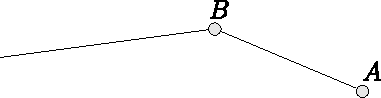
\includegraphics[width=0.8\linewidth]{2004-v3g-08-yl.pdf}
\end{center}

\hint

\solu
Klotsile $A$ mõjuva hõõdejõu kompenseerib nööri pinge, sestap on need kaks jõudu samasihilised ning klotsi $A$ juures peab pöörleva aluse kiirusvektor olema nööri sihiline. Pöörlemiskese peab lebama punktist $A$ tōmmatud lõigu $A B$ ristsirgel, pöörlemiskeskme $O$ leiame tingimusest $|\mathrm{OA}|=|\mathrm{AB}|$. Edasi on jooniselt lihtne mõõta $|OB|$ ning leida $b=a|O B| /|O A|=\SI{14}{cm}$. Klotsile $B$ mõjub hõõrdejõud, mille siht on risti sirgega $O B$. Samuti mõjub talle mõlema niidi pinged, mis on paralleelsed vastavate niitidega. Märgime punkti $C$ teisel niidil ning jagame vektori $\overrightarrow{B C}$ (mis kujutab teatud mõõtkavas selle niidi pinget) kaheks komponendiks, mis on paralleelsed kahe ülejäänud jõuga, $\overrightarrow{B C}=\overrightarrow{B D}+\overrightarrow{B E}$. Siinjuures lõik $B D$ on risti lõiguga $O B$ ja lõik $B E$ on paralleelne lõiguga $A B$. Et niidi $A B$ pinge on võrdne klotsile $A$ mõjuva hõõrdejõuga ja hõõrdejõudude suhe annab masside suhte, siis $m_{B}=m_{A}|B D| /|B E| .$ Jooniselt leiame $m_{B}=\SI{1,8}{g}$

\probend